
\documentclass[english,12pt,a4paper,pdftex]{article}
%% This package is required
%% Choose your school from arts, biz, chem, elec, eng, sci.
%% Choose the character encoding scheme used by your editor: utf8, latin1

\usepackage[elec,utf8]{aaltothesis} % this is the default in aaltothesis.sty
%% Use this if you run pdflatex and use jpg/pdf-format pictures.

\usepackage{graphicx}

%% Use the macros in this package to change how the hyperref package below 
%% typesets its hypertext -- hyperlink colour, font, etc. See the package
%% documentation. It also defines the \url macro, so use the package when 
%% not using the hyperref package.
%\usepackage{url}

%% Use this if you want to get links and nice output with pdflatex
\usepackage[pdfpagemode=None,colorlinks=true,urlcolor=red,%
linkcolor=blue,citecolor=black,pdfstartview=FitH]{hyperref}

%% Use this if you write hard core mathematics, these are usually needed
\usepackage{amsfonts,amssymb,amsbsy}  

%% Horizontal margins, DO NOT TOUCH!
\setlength{\hoffset}{-1in}
\setlength{\oddsidemargin}{35mm}
\setlength{\evensidemargin}{25mm}
\setlength{\textwidth}{15cm}
%% Vertical margins, DO NOT TOUCH!
\setlength{\voffset}{-1in}
\setlength{\headsep}{7mm}
\setlength{\headheight}{1em}
\setlength{\topmargin}{25mm-\headheight-\headsep}
\setlength{\textheight}{23cm}

%% Output starts here
\begin{document}
%% Change the school field to describe your school if the autimatically 
%% set name is wrong
% \university{aalto University}{aalto-Yliopisto}
% \school{School of Electrical Engineering}{SähköTekniikan korkeakoulu}

%% Vain kandityölle: Korjaa seuraavat vastaamaan koulutusohjelmaasi
%%
%% Only for B.Sc. thesis: Choose your degree programme. 
%\degreeprogram{Electronics and electrical engineering}%

%% Only for M.Sc. and Licentiate thesis: Choose your department,
%% professorship and professorship code. 
\department{Department of Signal Processing and Acoustics}%
{Signaalinkäsittelyn ja akustiikan laitos}
\professorship{Speech and Language Processing}{}
\code{S-89}

%% Choose one of these:
%\univdegree{BSc}
%\univdegree{MSc}
%% Added by Jose: For the non-finnish/swedish, the Lic degree is half of a PhD.
%\univdegree{Lic}
%% Add by Jose: For engineering exchange students (old plan, not Bolonia), PFC in Spain
%% IMPORTANT: FPr is only valid with English!!!
\univdegree{FPr}
%% Should be self explanatory...
\author{Jose Mariano Moreno Pimentel}

%% Your thesis title. If the title is very long and the latex 
%% does unsatisfactory job of breaking the lines, you will have to
%% break the lines yourself with \\ control character. 
%% Do not hyphenate titles.
\thesistitle{Text-to-Speech adaptation using noisy data}{}

\place{Espoo}
%% For B.Sc. thesis use the date when you present your thesis. 
\date{31.03.2014}

%% B.Sc. or M.Sc. thesis supervisor 
%% Note the "\" after the comma. This forces the following space to be 
%% a normal interword space, not the space that starts a new sentence. 
\supervisor{Prof.\ Mikko Kurimo}{Prof.\ Mikko Kurimo}

%% B.Sc. or M.Sc. thesis advisors(s). 
%%
%% Note that there has been a change in the official EN translation
%% of the Finnish title ``ohjaaja'' which in the previous version (1.5) 
%% of this document was called ``instructor''. The recommended
%% translation is now ``advisor''.  
%% However, the LaTeX internal variable remains \instructor
%% as there is little point to change the variable name. 
%%
%\instructor{Prof. Pirjo Professori}{Prof. Pirjo Professori}
%\instructor{D.Sc.\ (Tech.) Olli Ohjaaja}{TkT Olli Ohjaaja}
\instructor{M.Sc.\ (Tech.) Reima Karhila}{DI Reima Karhila}

%% Aalto logo: syntax:
% \uselogo{aaltoRed|aaltoBlue|aaltoYellow|aaltoGray|aaltoGrayScale}{?|!|''}
%% Logo language is set to be the same as the document language.
\uselogo{aaltoBlue}{''}

%% Create the coverpage
\makecoverpage

%% Force new page so that English abstract starts from a new page
\newpage
%
%% English abstract, uncomment if you need one. 
%% 
%% Abstract keywords
\keywords{speech synthesis, synthetic speech, TTS, HMM, noise robust, TTS adaptation}
%% Abstract text
\begin{abstractpage}[english]
 Your abstract in English. Try to keep the abstract short, approximately 
 100 words should be enough. Abstract explains your research topic, 
 the methods you have used, and the results you obtained.  
\end{abstractpage}
%% Note that 
%% if you are writting your master's thesis in English place the English
%% abstract first followed by the possible Finnish abstract

%% Preface
%\mysection{Esipuhe}
\mysection{Acknowledgments}

\vspace{5cm}
Otaniemi, 24.9.2013

\vspace{5mm}
{\hfill Jose M.\ Moreno \hspace{1cm}}

%% Force new page after preface
\newpage

%% Table of contents. 
\thesistableofcontents

\newpage
%% List of figures
\listoffigures

\newpage
%% List of tables
\listoftables

%% Symbols and abbreviations
\mysection{Symbols and abbreviations}
\subsection*{Symbols}

\subsection*{Opetators}

\subsection*{Abbreviations}
\begin{tabular}{ll}
	HMM			& Hidden Markov Model\\
	LP			& Linear Prediction\\
	LPC 		& Linear Predictive Coding\\
	LSP			& Line Spectral Pair\\
	STRAIGHT	& Speech Transformation and Representation using Adaptive \\
				& Interpolation of weiGHT spectrum\\
	TTS			& Text-To-Speech
\end{tabular}
%% Corrects the page numbering, there is no need to change these
\cleardoublepage
\storeinipagenumber
\pagenumbering{arabic}
\setcounter{page}{1}

\section{Introduction}
\label{intro}
\thispagestyle{empty}

Speech synthesis is not a recent ambition in mankind history. The earliest attempts to synthesize speech are only legends starring Gerbert d'Aurillac (died 1003 A.D.), also known as Pope Sylvester II. The pretended system used by him was a brazen head: a legendary automaton imitating the anatomy of a human head and capable to answer any question. Back in those days, the brazen heads were said to be owned by wizards. Following Pope Sylvester II, some important characters in mankind history  were reputed to have one of these heads, such as Albertus Magnus or Roger Bacon.

During the 18th century, Christian Kratzenstein, a German-born doctor, physicist and engineer working at the Russian Academy of Sciences, was able to built acoustics resonators similar to the human vocal tract. He activated the resonators with vibrating reeds producing the the five long vowels: /a/, /e/, /i/, /o/ and /u/.

Almost at the end of the 18th century, in 1791, Wolfgang von Kempelen presented his Acoustic-Mechanical Speech Machine \cite{vonKempelen}, which was able to produce single sounds and some combinations. During the first half of the 19th century, Charles Wheatstone built his improved and more complicated version of Kempelen's Acoustic-Mechanical Speech Machine, capable of producing vowels, almost all the consonants, sound combinations and even some words.	

In the late 1800's, Alexander Graham Bell also built a speaking machine and did some questionable experiments changing with his hands the vocal tract of his dog and making the dog bark in order to produce speech-like sounds \cite{Schroeder93}.


\section{History of Speech Synthesis}
\label{history_speech_synthesis}
Speech synthesis can be defined as the artificial generation of speech. Nowadays the process has been facilitated due to the improvements made during the last 70 years in computer technology, making the computer-based speech synthesis systems lead the way supported by their flexibility and their easier access compared to mechanical systems. However, after the first resonators built by Kratzenstein, the fist speaking machine was built and presented to the world in 1791, and was obviously mechanic.

\subsection{Acoustical-Mechanical Speech Machines}
The speech machine developed by von Kempelen incorporated models of the lips and the tong, enabling it to produce some consonants as well as vowels. Although Kratzenstein presented his resonators before von Kempelen his speech machine, von Kempelen started his work quite before, publishing a book where he described the studies made on human speech production and the experiments he made with his speech machine over 20 years of work \cite{vonKempelen}.  

The machine was composed by a pressure chamber, acting as lungs, a vibrating reeds in charge of the functions of the vocal cords and a leather tube that was manually manipulated in order to change its shape as the vocal tract does in an actual person, producing different vowel sounds. It had four separate constricted passages, controlled by the fingers, to generate consonants. Von Kempelen also included in his machine a model of the vocal tract with a hinged tongue and movable lips so as to create plosive sounds \cite{Schroeder93, LemmettyMSc, flanagan_1973_speech}. 



\begin{figure}[htb]
	\begin{center}
		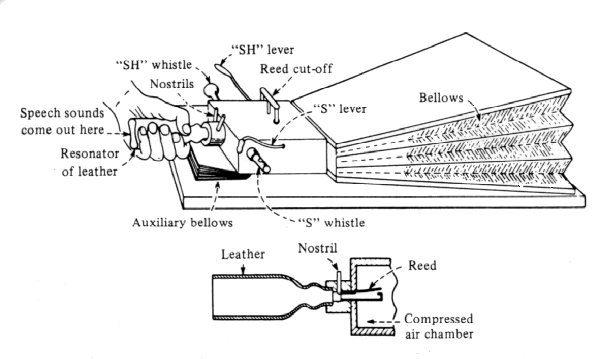
\includegraphics[width=\textwidth]{images/von_kempelen_machine.jpg}
		\caption{\cite{flanagan_book}}
	\end{center}
\end{figure}
\section{Speech Synthesis Systems}
\label{speec_synthesis_systems}
In this project we will use a HMM-based TTS system, but there are many different speech synthesis systems with their own advantages and disadvantages. In this section we will introduce the general architecture of a TTS system and diverse synthesis methods.

\subsection{TTS Architecture}
\label{speech_synthesis_systems_tts}
The main goal of a TTS system is to synthesize utterances from an arbitrary text. It is easy to notice that synthesizing from a text gives an extra flexibility to a synthesis system by allowing any reasonable input, in comparison to limited output systems such as GPS (Global Positional System) devices, but also an extra work has to be done to transform that text into the phonetic units required as inputs by the synthesizer. A general diagram of a TTS system is shown in Figure \ref{fig:tts_architecture}.

\begin{figure}[htb]
	\begin{center}
	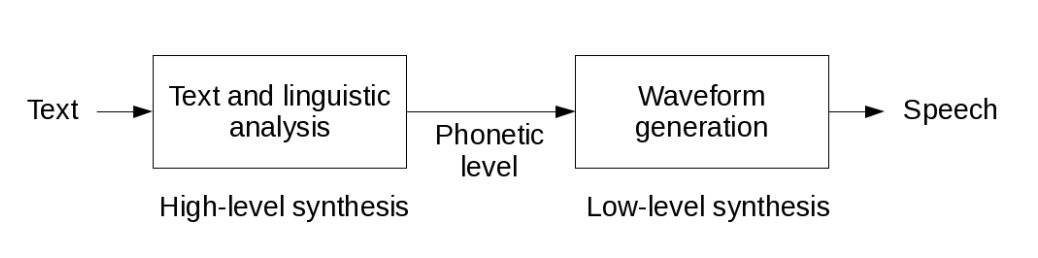
\includegraphics[width=\textwidth]{images/tts_architecture.jpg}
	\caption{General block diagram of a TTS system \cite{TuomoMSc}}
	\label{fig:tts_architecture}
	\end{center}
\end{figure}

The block representing the text and linguistic analysis is what differences a TTS system from other speech synthesis systems. The analysis made to the text has to generate the phonetic representation needed by the next component and predicting the desired prosody. Defining a larger set of goals for the speech synthesis system implies a more complex text and linguistic analysis. For example, trying to imitate the speaking style used by sports broadcaster in stead of synthesizing speech in a neutral style needs an extra function aiming to figure out the style of the input text, besides having constructed the corresponding model capable of producing speech mimicking the target style.

The main path followed by the text analysis includes a mandatory text normalization module. It is very important to normalize the text before trying to obtain its phonetic representation, to transform numbers, dates, acronyms and all the particularities that a language admit into a standardized form, called full-context labels representing the utterance on a phonetic-unit level based on the relations between phonemes, stress of each word, etc., accepted by the system. Also, this module is in charged of defining how similar spelled words are pronounced, e.g. the verb read has to different pronunciations whether is in the present tense or in the past tense. As it can be seen, text normalization is a complex problem that many researchers are looking for a solution to. An interesting approach to convert non-standard words (NSWs) into pronounceable words based on a taxonomy built from several text types is discussed in \cite{Sproat2001}.

Once the text is normalized, i.e. converted to plain letters, the structural properties of the text are analyzed and it is converted to a phonetic level. This last conversion is called the letter-to-sound conversion \cite{Pickett1999}. 

When the input text has gone through the first block represented in Figure \ref{fig:tts_architecture}, the low-level block generates predicts, based on the structural information and the prosodic analysis and tipically using statistical models, the fundamental frequency contour and phone durations. Finally, the speech waveform is generated by the vocoder. 

\subsection{Speech Synthesis Methods}
\label{speech_synthesis_systems_methods}
The generation of the waveform can be carried out in several ways, thus, we can talk about different speech synthesis methods. As written in \cite{TuomoMSc}, the different methods can be divided in two categories attending to whether the speech is generated from parameter, i.e. completely artificial, or real speech samples are used during the process. From all the methods explained in this section, only concatenative synthesis uses real samples to synthesize speech.

\subsubsection{Formant Synthesis}
\label{formant_speech_synthesis}
Formant synthesis is the most basic acoustic speech synthesis method. Based on the source-filter theory, which states that the speech signal can be represented in terms of source and filter characteristics \cite{Fant1970}, models the vocal tract with individually adjustable formant filters. The filters can be connected in serial, parallel or both. The different phonemes are generated by adjusting the center frequency, gain and bandwidth of each filter. Depending on the time intervals taken to do the adjustment, continuous speech can be generated. The source is modelled with voice pulses or noise.

Dennis Klatt's publication of the Klattalk synthesizer (see Section \ref{history_vocoder}) was the biggest boost received by formant synthesis. However, nowadays the quality given by this kind of synthesizers is lower than other newer methods, such as concatenative systems. Even so, formant synthesis is used in many applications such as reading machines for blind people, thanks to its intelligibility \cite{Pickett1999}.

\subsubsection{Articulatory Synthesis}
\label{articulatory_speech_synthesis}
The aim of articulatory synthesis is to model the human articulatory system as accurately as possible, using computational physical models. Therefore, this is theoretically the best method in order to achieve high-quality synthetic voices. However, modelling as accurately as possible raises the difficulty. The main setbacks are the difficult implementation needed in an articulatory speech synthesis system and the computational load, limiting this technique nowadays. Despite its currently limitations, articulatory models are being steadily developed and computational resources are still increasing, revealing a promising future.

\subsubsection{Concatenative Synthesis}
\label{concatenative_speech_synthesis}
Concatenative methods use prerecorded samples of real speech to generate the synthetic speech. It is easy to deduce that concatenative synthesis stands out from other methods of synthesis in terms of naturalness of individual segments. There are several unit lengths, such as word, syllable, phoneme, diphone, etc, that are smoothly combined to obtain the speech according to the input text. 

The main problem when using concatenative synthesis are the memory requirements. It is almost impossible to store all the necessary data for various speakers and contexts, making this technique the best one to imitate one specific speaker with one voice quality, but also makes it less flexible. It is difficult to implement adaptation techniques to obtain a different speaking style or a different speaker in concatenative speech. Apart from the storage problem, that thanks to the decrease in cost of digital storage and database techniques is becoming less serious, the discontinuities found in the joining points may cause some distortion even though the use of smoothing algorithms.

Concatenative systems may be the most widely used nowadays, but due to the limitations before commented, above all the flexibility problem, they might not be the best solution.

\subsubsection{LPC-Based Synthesis}
\label{lpc_based_speech_synthesis}
As in formant synthesis, in LPC-based synthesis utilizes source-filter theory of speech production. However, in this case the filter coefficients are estimated automatically from a short frame of speech, while in formant synthesis the different parameters are found for individual formant filters. Depending on the segment to be synthesized, the excitation needed is either a periodic signal, when synthesizing voiced segments, or noise, in case the segment is unvoiced. 

Linear Prediction (LP) has been applied in many different fields for a long time and was first used in speech analysis and synthesis in 1967. The idea is to predict a sample data by a linear combination of the previous samples. However, LPC targets not to predict any samples, but to represent the spectral envelope of the speech signal. 

Though the quality of basic LPC vocoder is consider poor, the more sophisticated LPC-based methods can produce high quality synthetic speech. The type of excitation is very important in LPC-based systems \cite{TuomoMSc}, but the strength of this method lays on its accuracy estimating the speech parameters and a relatively fast computational speed.

\subsubsection{HMM-Based Synthesis}
\label{hmm_based_speech_synthesis}
The use of HMMs in speech synthesis is becoming more popular. HMM-synthesis uses a statical model for describing speech parameters extracted from a speech database. Once the statistical models are built, they can be use to generate parameters according a text input that will be use for synthesizing. 

HMM-based synthesizers are able to produce different speaking styles, different speakers and even emotional speech. Other benefits are a smaller memory requirement and better adaptability. This last benefit is very interesting to us. While working with noisy data, limiting the amount of corrupted data used to train the system will probably affect positively to the quality of the synthetic speech obtained. Thus, constructing a high-quality average model and then taking profit of the adaptability of these systems to use the noisy data to train the adaptation transforms seems the correct approach. The data needed to train the adaptation transforms is always much lower than the training data used to built the average voice model.

On the other hand, naturalness is usually lower in HMM-based systems. But it must be said that these systems are improving very fast the quality of the synthetic speech obtained in terms of naturalness. 

As in this project we will be using HMM-based TTS systems, they are going to be described with more detail in Section \ref{hmm_synthesis}.

\section{Vocoders}
\label{vocoders}
The interface with both the natural speech and the synthesized speech is the vocoder. In this section, the fundamentals of the vocoder are presented and a detailed description of the two vocoders compared in this project is given.

\subsection{Vocoder}
\label{vocoders_vocoder}
The human speech is produced by regulating the air from the lungs through the 
%\section{Introduction}

%% Leave first page empty
%\thispagestyle{empty}

%% In a thesis, every section starts a new page, hence \clearpage
%\clearpage



%% Three levels of hierarchy in sectioning should be enough

\clearpage

%% The \phantomsection command is nessesary for hyperref to jump to the 
%% correct page, in other words it puts a hyper marker on the page.

\phantomsection
%\addcontentsline{toc}{section}{Viitteet}
\addcontentsline{toc}{section}{References}
\bibliographystyle{ieeetr}
\bibliography{sections/references}



\appendix 
\clearpage
%% Adds the word "Appendices" to the table of contents
\addtocontents{toc}{\protect\contentsline{section}{Appendices}{}{appendix}}

 %% appendix example (starts with section) in Finnish

%% Equations, tables and figures have their own numbering in Appendices, REMEMBER TO DO EVERY TIME YOU START AN APPENDIX, THE LETTER A IS THE APPENDIX INDEX
\renewcommand{\theequation}{A\arabic{equation}}
\setcounter{equation}{0}  
\renewcommand{\thefigure}{A\arabic{figure}}
\setcounter{figure}{0}
\renewcommand{\thetable}{A\arabic{table}}
\setcounter{table}{0}


\end{document}
